\documentclass[aspectratio=169,professionalfonts]{beamer}

\usetheme{AnnArbor}
\usecolortheme{dolphin}
\setbeamertemplate{navigation symbols}{}
\setbeamertemplate{footline}[frame number]

\usepackage{fontspec}
\setsansfont{Noto Sans}
\setmonofont{Noto Sans Mono}
\usepackage{booktabs}
\usepackage{array}
\usepackage{tabularx}
\usepackage{tikz}
\usetikzlibrary{positioning,arrows.meta,shapes.geometric}
\usepackage{listings}
\usepackage{xcolor}

\definecolor{sqlbg}{RGB}{248,248,248}
\definecolor{sqlkw}{RGB}{20,70,150}
\definecolor{sqlcm}{RGB}{90,90,90}
\definecolor{accent}{RGB}{0,89,156}

\lstdefinestyle{sqlstyle}{
  language=SQL,
  basicstyle=\ttfamily\scriptsize,
  keywordstyle=\color{sqlkw}\bfseries,
  commentstyle=\color{sqlcm},
  backgroundcolor=\color{sqlbg},
  frame=single,
  rulecolor=\color{black!20},
  columns=fullflexible,
  keepspaces=true,
  showstringspaces=false,
  breaklines=true,
  xleftmargin=0.5em,
  xrightmargin=0.5em,
  aboveskip=0.4em,
  belowskip=0.2em
}

\newcommand{\code}[1]{\texttt{#1}}
\newcommand{\smallnote}[1]{\vspace{0.3em}{\scriptsize\color{black!65}#1}}

\title[MySQL classicmodels]{MySQL Sample Database: \code{classicmodels}}
\subtitle{Introductory Tutorial on the MySQL Sample Database}
\author{DSAI1002 -- Database Practice}
\institute{Faculty of Data Science \& Artificial Intelligence}
\date{2026}

\begin{document}

\begin{frame}
  \titlepage
  \smallnote{Content Source: MySQL Tutorial -- MySQL Sample Database.}
\end{frame}

\section{Introduction}

\begin{frame}{Learning Objectives}
After this lesson, learners will be able to:
\begin{enumerate}
  \item Understand what \code{classicmodels} is and why it is commonly used for learning MySQL.
  \item Identify the primary data groups in the database.
  \item Understand the roles of key tables within the schema.
  \item Read the ER Diagram to trace relationships between tables.
  \item Set up the sample database to practice subsequent MySQL lessons.
\end{enumerate}
\end{frame}

\begin{frame}{What is the \code{classicmodels} Database?}
\begin{block}{Core Concept}
\code{classicmodels} is a sample database modeling a retail business that sells scale model classic vehicles.
\end{block}
\vspace{0.4em}
This database contains business operations data resembling real-world enterprise systems, making it ideal for practicing SQL queries from foundational to advanced levels.
\end{frame}

\begin{frame}{Data Groups in \code{classicmodels}}
\begin{columns}[T,onlytextwidth]
\column{0.48\textwidth}
\begin{itemize}
  \item Customers
  \item Products
  \item Product lines
  \item Sales orders
  \item Order details (line items)
\end{itemize}
\column{0.48\textwidth}
\begin{itemize}
  \item Customer payments
  \item Employees
  \item Sales offices
  \item Reporting structure
\end{itemize}
\end{columns}
\end{frame}

\begin{frame}{Why Use \code{classicmodels}?}
\begin{enumerate}
  \item More realistic and comprehensive than toy examples with only one or two tables.
  \item Well-suited for practicing \code{SELECT}, \code{WHERE}, \code{ORDER BY}, \code{GROUP BY}, \code{JOIN}, subqueries, views, and stored procedures.
  \item Features realistic primary key--foreign key relationships across multiple tables.
  \item Easily maps to real business analysis questions: top-spending customers, best-selling products, revenue by country, and unpaid orders.
\end{enumerate}
\end{frame}

\section{Installing the Sample Database}

\begin{frame}{Downloading the Sample Database}
\begin{itemize}
  \item Download the sample package from the MySQL Tutorial website.
  \item The package is typically compressed:
\end{itemize}
\begin{center}
\fbox{\Large\code{sampledatabase.zip}}
\end{center}
\begin{itemize}
  \item Once downloaded, extract the archive to obtain the SQL script used for importing into MySQL Server.
\end{itemize}
\end{frame}

\begin{frame}{Extracting the Database File}
\begin{itemize}
  \item You can use an extraction utility such as \code{7-Zip}.
  \item After extraction, you will typically find:
\end{itemize}
\begin{center}
\fbox{\Large\code{mysqlsampledatabase.sql}}
\end{center}
\begin{block}{What does the SQL file contain?}
Commands to create the database, create tables, and populate them with sample data.
\end{block}
\end{frame}

\begin{frame}{Two Ways to Import into MySQL Server}
\begin{columns}[T,onlytextwidth]
\column{0.48\textwidth}
\begin{block}{Method 1}
Using the \code{mysql command-line client}
\end{block}
\begin{itemize}
  \item Fast and lightweight
  \item Ideal for users comfortable with the terminal
\end{itemize}
\column{0.48\textwidth}
\begin{block}{Method 2}
Using \code{MySQL Workbench}
\end{block}
\begin{itemize}
  \item Graphical and intuitive
  \item Ideal for beginners
\end{itemize}
\end{columns}
\end{frame}

\begin{frame}[fragile]{Method 1: Import via Command Line}
Assuming the SQL file is located in the \code{Downloads} folder:
\begin{lstlisting}[style=sqlstyle,language=bash]
mysql -u root -p < "C:\Users\YourName\Downloads\mysqlsampledatabase.sql"
\end{lstlisting}
\begin{itemize}
  \item \code{-u root}: Log in as user \code{root}.
  \item \code{-p}: Prompt for password.
  \item \code{<}: Redirect SQL file contents into MySQL for execution.
\end{itemize}
\end{frame}

\begin{frame}{Method 2: Import via MySQL Workbench}
\begin{enumerate}
  \item Open MySQL Workbench and connect to your MySQL Server.
  \item Navigate to the menu: \code{Server > Data Import}.
  \item Choose \code{Import from Self-Contained File} and select \code{mysqlsampledatabase.sql}.
  \item Click \code{Start Import}.
  \item Verify that schema \code{classicmodels} appears in the schemas panel.
\end{enumerate}
\end{frame}

\begin{frame}[fragile]{Verification After Import}
\begin{lstlisting}[style=sqlstyle]
SHOW DATABASES;
USE classicmodels;
SHOW TABLES;
\end{lstlisting}
\vspace{0.4em}
Upon successful import, the table list will include \code{customers}, \code{employees}, \code{offices}, \code{orders}, \code{orderdetails}, \code{payments}, \code{productlines}, and \code{products}.
\end{frame}

\section{Schema and ERD}

\begin{frame}{Core Tables in the Schema}
\small
\begin{tabularx}{\textwidth}{>{\ttfamily}l X}
\toprule
Table & Purpose \\
\midrule
customers & Stores customer account and profile data \\
products & Stores inventory list of scale model classic vehicles \\
productlines & Stores product categories and descriptions \\
orders & Stores sales order headers \\
orderdetails & Stores line item details for each order \\
payments & Stores customer payment transactions \\
employees & Stores employee directory and reporting hierarchy \\
offices & Stores sales office locations \\
\bottomrule
\end{tabularx}
\end{frame}

\begin{frame}{ER Diagram: High-Level Relationships}
\centering
\resizebox{0.84\textwidth}{!}{%
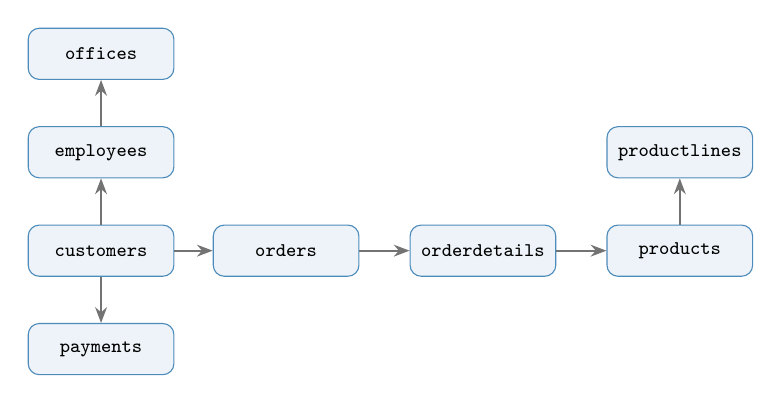
\begin{tikzpicture}[
  tbl/.style={rectangle, rounded corners, draw=accent!70, fill=accent!7, minimum width=1.85cm, minimum height=0.65cm, font=\scriptsize\ttfamily, align=center},
  rel/.style={-{Stealth[length=2mm]}, thick, draw=black!55}
]
\node[tbl] (customers) at (0,0) {customers};
\node[tbl] (orders) at (2.35,0) {orders};
\node[tbl] (orderdetails) at (4.85,0) {orderdetails};
\node[tbl] (products) at (7.35,0) {products};
\node[tbl] (productlines) at (7.35,1.25) {productlines};
\node[tbl] (payments) at (0,-1.25) {payments};
\node[tbl] (employees) at (0,1.25) {employees};
\node[tbl] (offices) at (0,2.50) {offices};

\draw[rel] (customers) -- (orders);
\draw[rel] (orders) -- (orderdetails);
\draw[rel] (orderdetails) -- (products);
\draw[rel] (products) -- (productlines);
\draw[rel] (customers) -- (payments);
\draw[rel] (customers) -- (employees);
\draw[rel] (employees) -- (offices);
\end{tikzpicture}%
}
\smallnote{Simplified diagram; the \code{employees} table also includes a self-referencing relationship \code{reportsTo}.}
\end{frame}

\begin{frame}{Customer and Product Tables}
\footnotesize
\begin{block}{\code{customers}}
Customer ID, customer name, contact details, address, country, sales representative, credit limit.
\end{block}
\vspace{0.45em}
\begin{block}{\code{products}}
Product code, product name, product line, scale, vendor, quantity in stock, buy price, MSRP.
\end{block}
\vspace{0.45em}
\begin{block}{\code{productlines}}
Product categories: Classic Cars, Motorcycles, Planes, Ships, Trains, Vintage Cars, etc.
\end{block}
\end{frame}

\begin{frame}{Orders and Payments Tables}
\footnotesize
\begin{block}{\code{orders}}
Order number, order date, required date, shipped date, status, comments, customer number.
\end{block}
\vspace{0.45em}
\begin{block}{\code{orderdetails}}
Order number, product code, quantity ordered, price each, order line number.
\end{block}
\vspace{0.45em}
\begin{block}{\code{payments}}
Customer number, check/payment number, payment date, and paid amount.
\end{block}
\end{frame}

\begin{frame}{Employees and Offices Tables}
\begin{columns}[T,onlytextwidth]
\column{0.48\textwidth}
\begin{block}{\code{employees}}
Employee number, full name, email, job title, assigned office, and direct manager.
\end{block}
\column{0.48\textwidth}
\begin{block}{\code{offices}}
Office code, city, phone, address, state/province, country, and territory.
\end{block}
\end{columns}
\vspace{0.5em}
\begin{alertblock}{Important Note}
The \code{employees} table contains a self-referencing foreign key to represent the managerial hierarchy.
\end{alertblock}
\end{frame}

\section{Sample Queries}

\begin{frame}[fragile]{Quick Inspection Queries}
\begin{lstlisting}[style=sqlstyle]
USE classicmodels;

SHOW TABLES;

SELECT customerNumber, customerName, country
FROM customers
LIMIT 10;
\end{lstlisting}
\end{frame}

\begin{frame}[fragile]{Inspecting Products and Recent Orders}
\begin{lstlisting}[style=sqlstyle]
SELECT productCode, productName, productLine, buyPrice, MSRP
FROM products
LIMIT 10;

SELECT orderNumber, orderDate, status, customerNumber
FROM orders
ORDER BY orderDate DESC
LIMIT 10;
\end{lstlisting}
\end{frame}

\begin{frame}[fragile]{Computing Line Item Revenue}
\begin{lstlisting}[style=sqlstyle]
SELECT orderNumber,
       productCode,
       quantityOrdered,
       priceEach,
       quantityOrdered * priceEach AS lineRevenue
FROM orderdetails
LIMIT 10;
\end{lstlisting}
\begin{block}{Significance}
Each record in \code{orderdetails} represents a product within an order. Line item revenue is calculated as quantity ordered multiplied by unit price.
\end{block}
\end{frame}

\begin{frame}[fragile]{JOIN: Orders with Customer Names}
\begin{lstlisting}[style=sqlstyle]
SELECT o.orderNumber,
       o.orderDate,
       o.status,
       c.customerName
FROM orders o
JOIN customers c
  ON o.customerNumber = c.customerNumber
LIMIT 10;
\end{lstlisting}
\smallnote{The foreign key \code{customerNumber} links \code{orders} to \code{customers}.}
\end{frame}

\begin{frame}[fragile]{JOIN: Products with Product Lines}
\begin{lstlisting}[style=sqlstyle]
SELECT p.productCode,
       p.productName,
       p.productLine,
       pl.textDescription
FROM products p
JOIN productlines pl
  ON p.productLine = pl.productLine
LIMIT 10;
\end{lstlisting}
\smallnote{This query maps each product to its category description in \code{productlines}.}
\end{frame}

\begin{frame}[fragile]{GROUP BY: Revenue by Order}
\begin{lstlisting}[style=sqlstyle]
SELECT od.orderNumber,
       SUM(od.quantityOrdered * od.priceEach) AS totalRevenue
FROM orderdetails od
GROUP BY od.orderNumber
ORDER BY totalRevenue DESC
LIMIT 10;
\end{lstlisting}
\begin{block}{Mental Model}
Select grouping key $\rightarrow$ calculate aggregate metric $\rightarrow$ sort output.
\end{block}
\end{frame}

\begin{frame}{MySQL Topics Explored with \code{classicmodels}}
\small
\begin{tabularx}{\textwidth}{>{\bfseries}l X}
\toprule
Topic & Practical Example \\
\midrule
Basic SELECT & Retrieve customer and product catalogs \\
WHERE & Filter customers by country or credit limit \\
ORDER BY & Sort orders chronologically \\
GROUP BY & Calculate revenue per customer or order \\
JOIN & Connect customers with their orders \\
Subqueries & Identify customers with above-average purchase value \\
Views / Procedures & Build reporting summaries and reusable routines \\
Indexing & Optimize query performance on keys and filters \\
\bottomrule
\end{tabularx}
\end{frame}

\section{Practice and Review}

\begin{frame}{Exercise 1: Import Database}
\begin{block}{Task}
Import the \code{classicmodels} database into your MySQL Server instance.
\end{block}
Verify the setup using the following commands:
\begin{itemize}
  \item \code{SHOW DATABASES;}
  \item \code{USE classicmodels;}
  \item \code{SHOW TABLES;}
\end{itemize}
\end{frame}

\begin{frame}[fragile]{Exercise 2: Query the First 10 Customers}
Retrieve \code{customerNumber}, \code{customerName}, \code{city}, and \code{country}.
\begin{lstlisting}[style=sqlstyle]
SELECT customerNumber, customerName, city, country
FROM customers
LIMIT 10;
\end{lstlisting}
\end{frame}

\begin{frame}{Exercises 3--4: Products and Revenue}
\begin{block}{Exercise 3}
Query products belonging to the \code{Classic Cars} product line. Display \code{productCode}, \code{productName}, \code{productLine}, and \code{MSRP}.
\end{block}
\begin{block}{Exercise 4}
Calculate the total revenue for each order from \code{orderdetails} using \code{quantityOrdered * priceEach}, grouped by \code{orderNumber}.
\end{block}
\end{frame}

\begin{frame}{Exercise 5: JOIN Orders and Customers}
Write a JOIN query to display orders along with corresponding customer names.
\vspace{0.5em}
\begin{itemize}
  \item Table 1: \code{orders}
  \item Table 2: \code{customers}
  \item Join key: \code{customerNumber}
\end{itemize}
\end{frame}

\begin{frame}{Discussion Questions}
\begin{enumerate}
  \item What business model does the \code{classicmodels} database simulate?
  \item Why is \code{classicmodels} well-suited for learning relational databases?
  \item What role does the \code{orderdetails} table serve?
  \item Why is the \code{productlines} table separated from the \code{products} table?
  \item How does an ER Diagram help when working with \code{classicmodels}?
\end{enumerate}
\end{frame}

\begin{frame}{Multiple Choice Questions}
\small
\begin{enumerate}
  \item Which industry domain does \code{classicmodels} model?\newline
  A. Scale model classic car retail \quad B. Hospital management \quad C. Digital library \quad D. Social network
  \item Which table stores customer data?\newline
  A. \code{products} \quad B. \code{customers} \quad C. \code{orders} \quad D. \code{offices}
  \item Which table stores line items within each order?\newline
  A. \code{payments} \quad B. \code{employees} \quad C. \code{orderdetails} \quad D. \code{productlines}
  \item Which table records customer payment transactions?\newline
  A. \code{products} \quad B. \code{orders} \quad C. \code{offices} \quad D. \code{payments}
\end{enumerate}
\end{frame}

\begin{frame}{Lesson Summary}
\begin{itemize}
  \item \code{classicmodels} is a widely used sample database in MySQL simulating a scale model vehicle retailer.
  \item The schema comprises \code{customers}, \code{products}, \code{productlines}, \code{orders}, \code{orderdetails}, \code{payments}, \code{employees}, and \code{offices}.
  \item It provides an ideal dataset for mastering \code{SELECT}, \code{JOIN}, \code{GROUP BY}, aggregations, views, and stored procedures.
  \item ER Diagrams help learners map entity relationships before composing SQL statements.
\end{itemize}
\end{frame}

\begin{frame}{Key Terms}
\centering
\Large
\code{MySQL} \quad \code{classicmodels} \quad \code{Schema} \\
\vspace{0.5em}
\code{ER Diagram} \quad \code{SELECT} \quad \code{JOIN} \\
\vspace{0.5em}
\code{GROUP BY} \quad \code{View} \quad \code{Stored Procedure}
\end{frame}

\end{document}
